% GRASP: Copyright 1997,1998,1999  Bruce Allen %
% $Id: man_correlation.tex,v 1.4 1999/07/11 21:22:10 ballen Exp $
\section{GRASP Routines: Signal-to-noise enhancement techniques}
\label{s:correlation}
\setcounter{equation}0

\subsection{Signal-to-noise enhancement by environmental cross-correlation}
\setcounter{equation}0
\label{ss:cross-correlation}

There are many situations of interest in which data are contaminated
by the environment.  Often this contamination is understood, and by
monitoring the environment it is possible to ``clean up" or ``reduce"
the data, by subtracting the effects of the environment from the
signal or signals of interest.  In the case of the data stream from an
interferometric gravitational radiation detector, the signal of
interest is the differential displacement of suspended
test masses.  This displacement arises from gravitational waves but
also has contributions arising from other contaminating sources, such
as the shaking of the optical tables (seismic noise) and forces due to
ambient environmental magnetic fields.  The key point is that the
gravitational waves are not correlated with any of these environmental
artifacts.

The method implemented here works by estimating the linear transfer
function between the IFO\_DMRO channel and specified environmental
channels on the basis of the correlations over a certain bandwidth in
Fourier space.  The method is explained in detail in the paper
`\emph{Automatic cross-talk removal from multi-channel data}'
(WISC-MILW-99-TH-04)%
\footnote{available from
\htmladdnormallink{{\tt http://www.lsc-group.phys.uwm.edu/$\sim$www/docs/pub\_table/gravpub.html}}
{http://www.lsc-group.phys.uwm.edu/~www/docs/pub_table/gravpub.html}
.}
Here we will just give a very brief overview to introduce the quantities calculated.

We denote the channel of interest, normally the InterFerOmeter Differential
Mode Read-out (IFO\_DMRO), by $X$ or $Y_1$.  The other sampled channels consist
of environmental and instrumental monitors which we denote
$Y_2,\dots,Y_N$.  We assume that all fast channels have been decimated
so that all channels are sampled at the same (slow) rate,
$986.842\cdots\ $Hz for the November 1994 40-meter data.


We assume that the contribution of channel $i$ to channel $1$ is
described by an (unknown!) linear transfer function $R_i(t-t')$. The
basic idea of the method is to use the data to estimate the transfer
functions $R_i$.  For the reasons discussed in the paper, we work
with the data in Fourier space.  The transfer function is estimated by
averaging over a frequency band, that is a given number of frequency
bins.  The number of bins in any band is  denoted by $F$ in
the cited paper and {\tt correlation\_width} in
the programs below.  The method assumes that $\tilde R_i$ can be well
approximated by a {\it complex constant} within each frequency band,
in other words that the transfer function
does not vary rapidly over the frequency bandwidth $\Delta f = F/T$
where $T$ is total time of the data section under consideration.
The choices 32, 64 and 128 appear most appropriate for $F$ for the
40-meter data. 

Within a given band, $b$, the Fourier components of the field may be thought
of as the components of an $F$-dimensional vector, ${\bf Y}_i^{(b)}$.    
Correlation between two channels (or the auto-correlation of
a channel with itself) may be expressed by the standard inner product
$({\bf Y}_i^{(b)},{\bf Y}_j^{(b)}) = {\bf Y}_i^{(b)}{\cdot}{\bf
  Y}_j^{(b)*}$ (no summation over $b$). Our assumption that $\tilde R_i$
is constant over each band means that the `true' channel of interest
(the IFO\_DMRO channel with environmental influences subtracted) can
be written
\begin{equation}
\bar {\tilde {\bf x}}^{(b)} =  {\tilde {\bf X}}^{(b)} - \sum_{j=2}^N
r^{(b)}_j {\tilde {\bf Y}_j}^{(b)}.
\end{equation}
where $r^{(b)}_j$, $j=2,\dots,N$ are constants.
The fundamental assumption is that the best estimate of the transfer
function in the frequency band $b$ is given by the complex vector 
$(r^{(b)}_2,\dots,r^{(b)}_N)$ that minimises 
$|\bar {\tilde {\bf x}}^{(b)}|^2$.
To measure the `improvement' in the signal we define $|\rho|^2$ by
\begin{equation}
 |\bar {\tilde {\bf x}}^{(b)}|^2 = | {\tilde {\bf X}}^{(b)}|^2 
      \left( 1 - |\rho|^2 \right) .
\end{equation}
denoted by {\tt rho2} in the programs below.
By definition $0 \leq |\rho|^2 \leq 1$.
If any of the  environmental channels are strongly correlated
with the channel of interest, a significant reduction in  
$|\bar {\tilde {\bf x}}^{(b)}|^2$ is
obtained, that is, $|\rho|^2$ will be close to 1.

To understand the origin of the `improvement' it is also convenient to
study the best estimate that can be obtained using any given single
environmental channel.  Thus we define 
\begin{equation}
\bar {\tilde {\bf x}}^{(b)}_i
=  {\tilde {\bf X}}^{(b)} - 
{r'}^{(b)}_i {\tilde {\bf Y}_i}^{(b)}
\end{equation}
and choose the complex number ${r'}^{(b)}_i$ to  minimise 
$|\bar {\tilde {\bf x}}^{(b)}_i|^2$.  Of course, in general this
will not correspond to the $i$th component of the vector 
used in the multi-channel case.
The corresponding improvement $|\rho_i|^2$ given by 
\begin{equation}
|\bar {\tilde {\bf x}}^{(b)}_i|^2 = |{\tilde {\bf X}}^{(b)}|^2 
      \left( 1 - |\rho_i|^2 \right)
\end{equation}
is denoted by {\tt rho2\_pairwise} in the programs below.
By definition $0 \leq |\rho_i|^2 \leq 1$.
If the $i$th  environmental channel is  strongly correlated
with the channel of interest, a significant reduction in  
$|\bar {\tilde {\bf x}}^{(b)}_i|^2$ is
obtained, that is, $|\rho_i|^2$ will be close to 1.
 



\clearpage
\subsection{Outline}

Calculation of environmental correlations using the routines presented
in this chapter proceeds through the 
establishment of a configuration file, called here {\tt 40m.config} 
with the following structure:

\begin{verbatim}
#  Correlations between 40m Channels  over a period
#  of approximately 266 seconds. The IFO sample rate is 
#  9868.4\dots Hz (hence 9868.4 x 266 = 2621440 samples).
#  The sample rate for the `slow' channels is
#  (1/10)th that of the `fast' so (1/10)th the
#  number of samples are requested 
C1
4
IFO_DMRO        S        2621440
IFO_Mike        S        2621440
IFO_Seis_1      S        262144
IFO_SPZT        S        262144
1
\end{verbatim}

  The file may {\it begin} with any number of comment lines beginning
with an initial {\tt \#}.  The next line is a character string 
describing the detector, this is just used for naming intermediate files.
The following line gives the total number of channels (signal plus
environmental).  There follow this number of lines each containing
three columns, the first of these lines pertains to the signal 
the remainder to environmental channels.  The three columns are:
\begin{enumerate}
\item the name of the channel,
\item the data type of the channel (here short) -- see {\tt
animateT.c} or {\tt corr\_init.c} for a description of the possible types,
and 
\item the number of data points from that channel to be analysed --
these should correspond to the same period of time.
\end{enumerate}


\noindent Finally, there is a line containing a single number.  This should be
set to 1 if the user wants to obtain `cleaned' output and 0 if the
user just wants to see correlation data.  (Note: This line is not used by
{\tt corr\_init} described below, but only by {\tt env\_corr}.  Thus it
is possible to change one's mind about whether to find the cleaned 
signal without having to rerun {\tt corr\_init}.)

The configuration file is used by the two basic programs:
\begin{enumerate}
\item {\tt  corr\_init} which calculates the Fourier transforms and writes 
binary data files in a data directory named {\tt `configuration name'\_fft}, so
{\tt 40m\_fft} in the above example. Only those frequencies
appropriate to the slowest channel are saved.
\item {\tt env\_corr} which calculates the correlations between each
environmental channel and the signal channel and pops up a graph 
of these correlations.  
The data for this graph is stored in the same data directory as the
FFT data.  {\tt env\_corr} also produces a file {\tt corr\_view\dots}
which enables this graph to be reproduced later without running  {\tt
  env\_corr} again.  If the configuration file asks for the
signal to be cleaned {\tt env\_corr} will also produce an ASCII data file
giving the (FFT of the) `cleaned' signal and also the total fractional reduction 
in noise obtained by the method. 
Again this file is stored in the same data directory, its first line
gives the frequency spacing and the following lines the real and
imaginary parts of the FFT of the cleaned signal.  (To avoid plotting
difficulties with {\tt xmgr} the DC component is arbitrarily set equal
to that of the first bin.)  
\end{enumerate}

Thus, having created the appropriate configuration file one would
type {\tt corr\_init  40m.config} and then {\tt env\_corr 40m.config}.
(Of course, the environment variable {\tt GRASP\_FRAMEPATH} must first
be set to the directory containing the appropriate frames.)

\begin{description}
\item{Note:} These programs perform linear algebra by calls to 
{\tt clapack} routines.  These may be obtained from {\tt
  http://www.netlib.org/}.  These routines use {\tt f2c} 
and, in particular, use complex numbers defined
in {\tt f2c.h} through the structure:

{\tt 
typedef struct \{\\
  float r;  /* real part */\\
  float i;  /* imaginary part */\\
\} complex;}

\end{description}

\clearpage
\subsection{Function: {\tt calc\_rho()}}
\setcounter{equation}0
{\tt int calc\_rho(int offset,int correlation\_width,float threshold,
               float *rp\_signal,\\float *ip\_signal,int nenv\_chan,
               float **rp\_env,float **ip\_env,\\ float *rho2\_pairwise,
               complex *A,complex *B,float *modx2sum)} 

This function takes sections of length {\tt length} of the Fourier
transform of the `signal' channel and {\tt nenv\_chan} environmental
channels and estimates the transfer function on the basis of
correlations over a width  of {\tt correlation\_width} bins at an
offset frequency of {\tt offset} bins.  It returns an array {\tt rho2\_pairwise}
containing the values of $|\rho|^2$ that would arise from a
cross-correlation with each single channel thereby giving information
on {\it which}
environmental channels contain the strongest evidence for correlation with 
the signal.

The arguments are:
\begin{description}
\item{\tt length:} Input. The total length of the Fourier transform.
\item{\tt offset:} Input. The offset to the beginning of the section
  of the Fourier transform over which correlations are being searched for.
\item{\tt correlation\_width:} Input.  The width of the section
  of the Fourier transform over which correlations are being searched for.
\item{\tt threshold:} Input. The threshold for determining whether a
correlation is statistically significant.
\item{\tt rp\_signal:} Input. {\tt  rp\_signal[0..length-1]} contains the
  real parts of the Fourier transform of the signal.
\item{\tt ip\_signal:} Input. {\tt  ip\_signal[0..length-1]} contains the
  imaginary parts of the Fourier transform of the signal.
\item{\tt nenv\_chan:} Input. The number of environmental channels under
  consideration.
\item{\tt rp\_env:} Input. {\tt  rp\_env[0..nenv\_chan-1][0..length-1]} contains the
  real parts of the Fourier transform of the nenv\_chan environmental channels.
\item{\tt ip\_env:} Input. {\tt  ip\_env[0..nenv\_chan-1][0..length-1]} contains the
  imaginary parts of the Fourier transform of the nenv\_chan environmental
  channels.
\item{\tt rho2\_pairwise:} Output. {\tt rho2\_pairwise[0..nenv\_chan-1]} contain
  the level of {\it pairwise} correlation between  the signal and each
  environmental channel in turn, {\it i.e.}, the value of $|\rho|^2$ 
  obtained if just the $i$th environmental channel had been used.
\item{\tt A:} Input/Output. {\tt A[0..${\tt nenv\_chan}^2$-1]} is a working
  array that is used by the {\sl clapack} routine {\tt chesv()} called by {\tt clean\_chan()}.  
  The elements of the array are structure of type {\tt complex} (see
  note above).  Memory allocation should be performed in the
  calling routine.
\item{\tt B:} Input/Output. {\tt B[0..${\tt nenv\_chan}$-1]} is a working
  array used by the {\sl clapack} routine {\tt chesv()} called by {\tt clean\_chan()}.  
  The elements of the array are structure of type {\tt complex} (see
  note above).  Memory allocation should  be performed in the
  calling routine.
\item{\tt modx2sum:} Output.  A float used by {\tt clean\_chan}.
\end{description}

\begin{description}
\item{Author:}
Bruce Allen (ballen@dirac.phys.uwm.edu), Wensheng Hua (hua@bondi.phys.uwm.edu)
  and Adrian Ottewill (ottewill@relativity.ucd.ie).
\item{Comments:}

\end{description}
\clearpage

\subsection{Function {\tt chan\_clean()}}

\setcounter{equation}0

{\tt int chan\_clean(int offset,int correlation\_width,float
  threshold,float *rho2,\\
float *rp\_signal,float *ip\_signal,
               int nenv\_chan,float **rp\_env,float **ip\_env,\\
float *rp\_clean,float *ip\_clean,complex *A,complex *B,\\
               float modx2sum,complex *R,complex *work,integer lwork,integer *ipivot)}

\begin{description}
\item{Note:} The data type {\tt integer} is defined in {\tt f2c.h}.
\end{description}

\begin{description}
\item{\tt offset:} Input. The offset to the beginning of the section
  of the Fourier transform over which correlations are being searched for.
\item{\tt correlation\_width:} Input.  The width of the section
  of the Fourier transform over which correlations are being searched for.
\item{\tt threshold:} Input. The threshold for determining whether a
correlation is statistically significant.
\item{\tt rp\_signal:} Input. {\tt  rp\_signal[0..length-1]} contains the
  real parts of the Fourier transform of the signal.
\item{\tt ip\_signal:} Input. {\tt  rp\_signal[0..length-1]} contains the
  imaginary parts of the Fourier transform of the signal.
\item{\tt nenv\_chan:} Input. The number of environmental channels under
  consideration.
\item{\tt rp\_env:} Input. {\tt  rp\_env[0.. nenv\_chan-1][0..length-1]} contains the
  real parts of the Fourier transform of the nenv\_chan environmental channels.
\item{\tt ip\_env:} Input. {\tt  ip\_env[0.. nenv\_chan-1][0..length-1]} contains the
  imaginary parts of the Fourier transform of the nenv\_chan environmental
  channels.
\item{\tt rp\_clean:} Output. {\tt  rp\_clean[0..length-1]} contains the
  real parts of the Fourier transform of the signal cleaned by
  removing those contributions that have been assigned by the method
  to environmental influences.
\item{\tt ip\_clean:} Output. {\tt  ip\_clean[0..length-1]} contains the
  imaginary parts of the Fourier transform of the signal cleaned by
  removing those contributions that have been assigned by the method
  to environmental influences.
\item{\tt A:} Input. {\tt A[0..${\tt nenv\_chan}^2$-1]} is a working
  array that is calculated by {\tt calc\_rho()} and used by the {\sl
  clapack} routine {\tt chesv()} called by {\tt clean\_chan()}.  
  The elements of the array are structure of type {\tt complex} (see
  note above).  Memory allocation should be performed in the
  calling routine.
\item{\tt B:} Input. {\tt B[0..${\tt nenv\_chan}$-1]} is a working
  array that is calculated by {\tt calc\_rho()} used by the {\sl
    clapack} 
routine {\tt chesv()} called by {\tt clean\_chan()}.  
  The elements of the array are structure of type {\tt complex} (see
  note above).  Memory allocation should  be performed in the
  calling routine.
\item{\tt modx2sum:} Input.  A float that is calculated by {\tt
    calc\_rho} used by {\tt clean\_chan}.
\item{\tt R:} Input. {\tt R[0..${\tt nenv\_chan}$-1]} is a working
  array used by the {\sl clapack} routine {\tt chesv()} called by {\tt clean\_chan()}.  
  The elements of the array are structure of type {\tt complex} (see
  note above).  Memory allocation should be performed in the
  calling routine. 
\item{\tt work:} Input. {\tt work[0..${\tt lwork}$-1]} is a working
  array used by the {\sl clapack} routine {\tt chesv()} called by {\tt clean\_chan()}.  
  The elements of the array are structure of type {\tt complex} (see
  note above).  Memory allocation should be performed in the
  calling routine. 
\item{\tt lwork:} Input. The size of the array {\tt work}.
\item{\tt ipivot:} Input. {\tt ipivot[0..${\tt nenv\_chan}$-1]} is a working
  array used by the {\sl clapack} routine {\tt chesv()} called by {\tt clean\_chan()}.  
  The elements of the array are structure of type {\tt integer}.  Memory
  allocation should be performed in the  calling routine. 
\end{description}
\begin{description}
\item{Author:}
Bruce Allen (ballen@dirac.phys.uwm.edu), Wensheng Hua (hua@bondi.phys.uwm.edu)
  and Adrian Ottewill (ottewill@relativity.ucd.ie).
\item{Comments:}
{\tt clean\_chan()} currently uses {\sl clapack} routines to
perform the required matrix manipulations.  While this it is highly
desirable to have such optimised routines when considering a large
number of environmental channels it would also be useful to have a replacement
for the {\sl clapack} routine {\tt chesv()} constructed from Numerical
Recipes routines for when {\sl clapack} is not available.
\end{description}

\clearpage




\subsection{Example: Correlations in data from the  40m interferometer }


 

The output below was produced starting with  2621440 samples from the 19
November 1994 run 3 data set, covering about 266 seconds.

The fast channels, including the IFO\_DMRO channel, were decimated
so that all channels are effectively sampled at the slow channel rate
of $986.842\dots\,$Hz. This yields a (real) time series with 262144
samples and correspondingly a (complex) FFT of length 131072 as
specified by the macro name {\tt LENGTH}.
Averaging is carried out over 128 frequency bins but this may
be varied to include a range of bandwidths  {\tt MIN\_BANDWIDTH} and {\tt MAX\_BANDWIDTH}. 

\begin{figure}[ht]
\index{colorpage}
\begin{center}
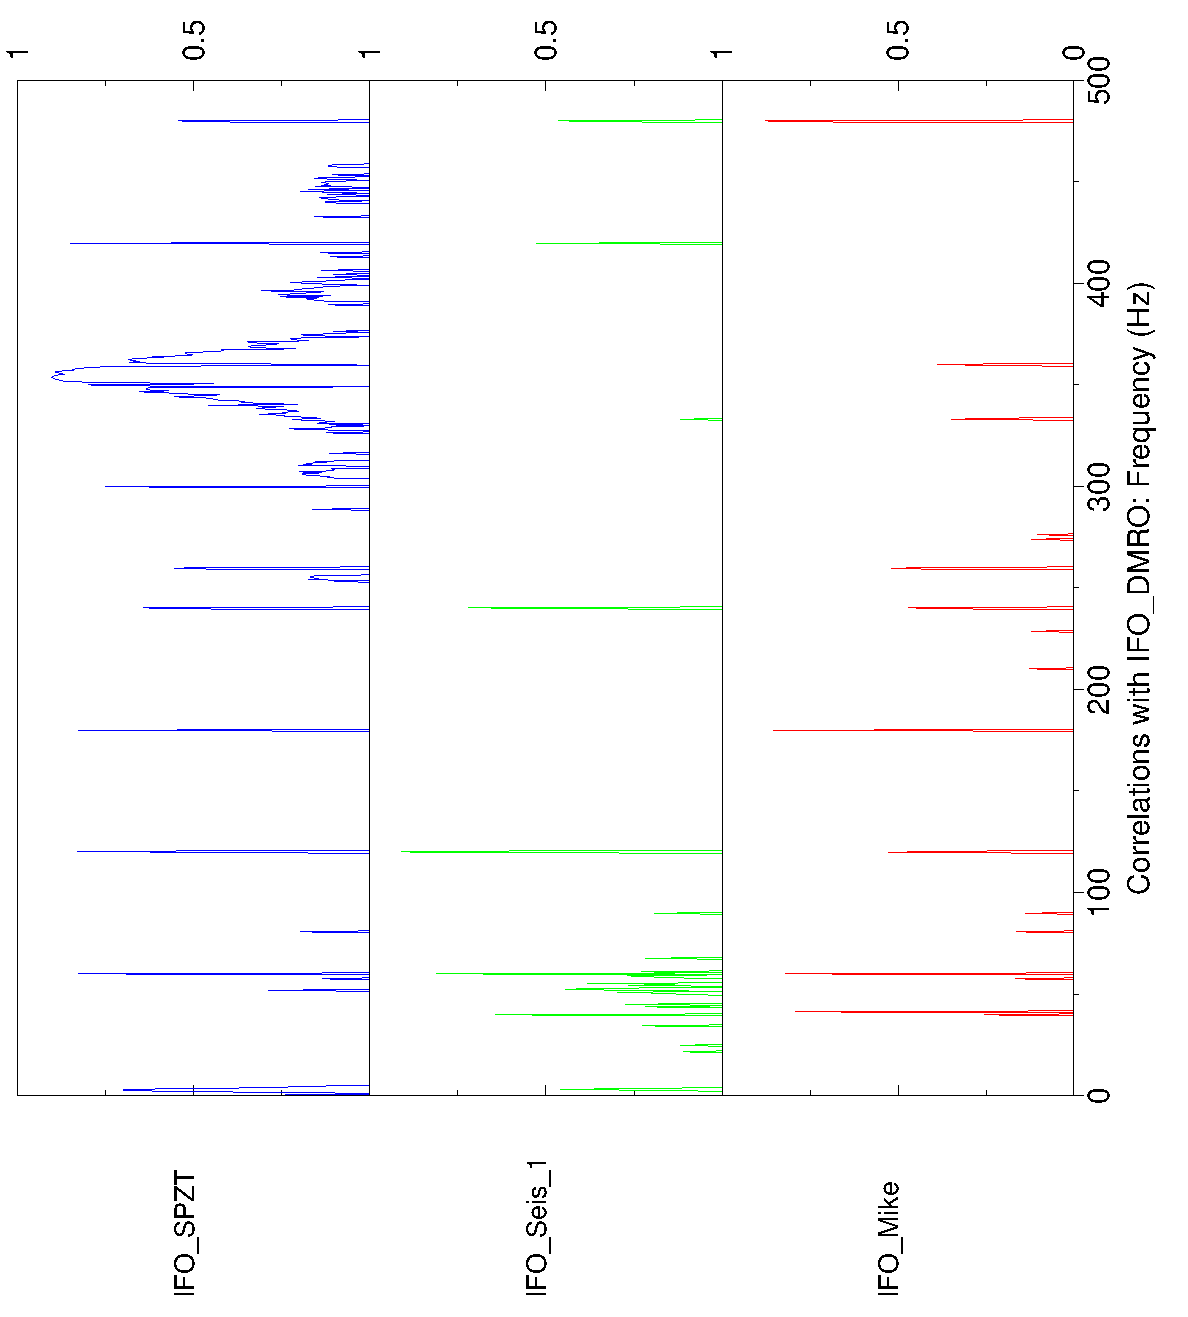
\epsfig{file=Figures/xmgr.eps,angle=270,width=5in}
\caption{ \label{f:rho2} The graphical display of the contents of the 
output file  {\tt 40m\_fft/rho2\_IFO\_128.dat} produced by {\tt env\_corr}
illustrating strong environmental cross-correlation.  
 The three graphs show the correlation between the
IFO\_DMRO channel and each individual environmental channel.
This graph is produced by the file {\tt corr\_view128} which {\tt
  env\_corr} produces.}

\end{center}
\end{figure}


The output was obtained from the commands

\centerline{\tt corr\_init 40m.config}

\noindent followed by

\centerline{\tt env\_corr 40m.config}

\noindent where  {\tt 40m.config} is the configuration file printed above.
This corresponding to seeking correlations between the
interferometer output (IFO\_DMRO) channel and 
\begin{description}
\item{IFO\_Mike:} The microphone output.
\item{IFO\_Seis\_1:} The seismometer output.
\item{IFO\_SPZT:} The slow pzt.
\end{description}

The data below show sections of the output file  {\tt 40m\_fft/rho2\_IFO\_128.dat}
illustrating strong environmental cross-correlation
at around $40$Hz with the seismometer and microphone output, at 
around $120$Hz with all three channels, and in a broad band 
around 360Hz with the slow pzt.

{\tt 
\begin{verbatim}
... 
39.271          0.000           0.000 0.000 0.000 
39.753          0.654           0.256 0.644 0.000 
40.235          0.000           0.000 0.000 0.000 
40.717          0.000           0.000 0.000 0.000 
41.199          0.794           0.794 0.000 0.000 
41.681          0.000           0.000 0.000 0.000 
...
118.778         0.000           0.000 0.000 0.000 
119.259         0.000           0.000 0.000 0.000 
119.741         0.940           0.528 0.876 0.519 
120.223         0.973           0.371 0.911 0.830 
120.705         0.000           0.000 0.000 0.000 
121.187         0.000           0.000 0.000 0.000 
...
352.478         0.886           0.000 0.000 0.886 
352.960         0.897           0.000 0.000 0.897 
353.442         0.899           0.000 0.000 0.899 
353.924         0.904           0.000 0.000 0.904 
354.405         0.898           0.000 0.000 0.898 
354.887         0.897           0.000 0.000 0.897 
355.369         0.869           0.000 0.000 0.869 
355.851         0.878           0.000 0.000 0.878 
356.333         0.893           0.000 0.000 0.893 
356.815         0.893           0.000 0.000 0.893 
357.297         0.843           0.000 0.000 0.843 
357.778         0.845           0.000 0.000 0.845 
...
\end{verbatim}}
\noindent

\begin{figure}[ht]
\index{colorpage}
\begin{center}
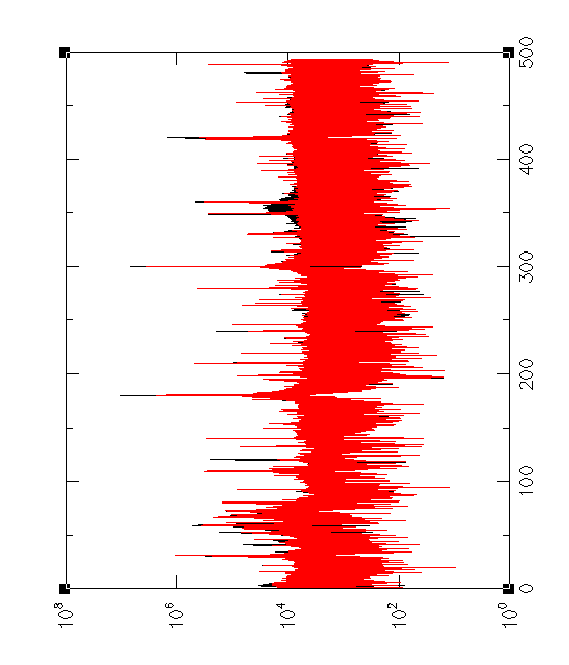
\epsfig{file=Figures/cleaned.eps,angle=270,width=5in}
\caption{ \label{f:cleaned} The spectrum of the IFO\_DMRO channel
before (black) and after `cleaning' based on the three environmental
channels  discussed in the text
using a correlation width of 128 bins (red).}
\end{center}
\end{figure}



The output file  {\tt 40m\_fft/fftclean\_IFO\_128.dat} contains the Fourier
transform  of the corresponding signal `cleaned'
by estimating the transfer functions over a correlation width of
128 bins. 
Figure~\ref{f:cleaned} shows the spectrum of the IFO\_DMRO channel
before and after `cleaning' based on environmental channels 1, 2 and 5.


\clearpage
\subsection{Example: {\tt corr\_init} }



This program calculates the FFTs of the various channels specified in
the configuration file and stores them in binary files in a
subdirectory of the working directory, whose name is determined by the
detector name specified in the configuration file.

\begin{description}
\item{Typical usage:} {\tt corr\_init 40m.config}
\end{description}

\lgrindfile{Includes/corr_init.tex}

\clearpage

\subsection{Example: {\tt env\_corr} }

This program calls {\tt calc\_rho} and {\tt clean\_chan} to determine
environmental correlations. It pops up a graph plotting these 
correlation as well as writing files containing data on the
correlations
and the `cleaned' signal.



\begin{description}
\item{Typical usage:} {\tt env\_corr  40m.config}
\end{description}

\lgrindfile{Includes/env_corr.tex}


\begin{description}
\item{Author:}
Bruce Allen (ballen@dirac.phys.uwm.edu), Wensheng Hua (hua@bondi.phys.uwm.edu)
  and Adrian Ottewill (ottewill@relativity.ucd.ie).
\item{Comments:} None.
\end{description}

\clearpage
